\documentclass[tikz,border=8pt]{standalone}
% Shared look for every TikZ diagram. Load with \input{../../tools/tikz-style.tex}
\usepackage[T1]{fontenc}
\usepackage{lmodern}
\renewcommand{\sfdefault}{lmr}  % diagrams use the same serif as the text
\usetikzlibrary{arrows.meta, positioning, shapes.geometric, calc, fit, backgrounds}
\definecolor{cblue}{HTML}{4C78A8}
\definecolor{corange}{HTML}{F58518}
\definecolor{cgreen}{HTML}{54A24B}
\definecolor{cred}{HTML}{E45756}
\definecolor{cpurple}{HTML}{B279A2}
\definecolor{cgrey}{HTML}{6B6B6B}
\tikzset{
  every picture/.style={font=\sffamily, line width=1.2pt},
  box/.style={draw=#1, fill=#1!12, rounded corners=4pt, align=center, inner sep=7pt, minimum height=1.1cm},
  box/.default=cgrey,
  arrow/.style={-{Stealth[length=3mm]}, draw=cgrey, line width=1.4pt},
  title/.style={font=\sffamily\bfseries\Large},
  note/.style={font=\sffamily\small, text=cgrey, align=center},
}
\AtBeginDocument{\hyphenpenalty=10000 \exhyphenpenalty=10000}

\begin{document}
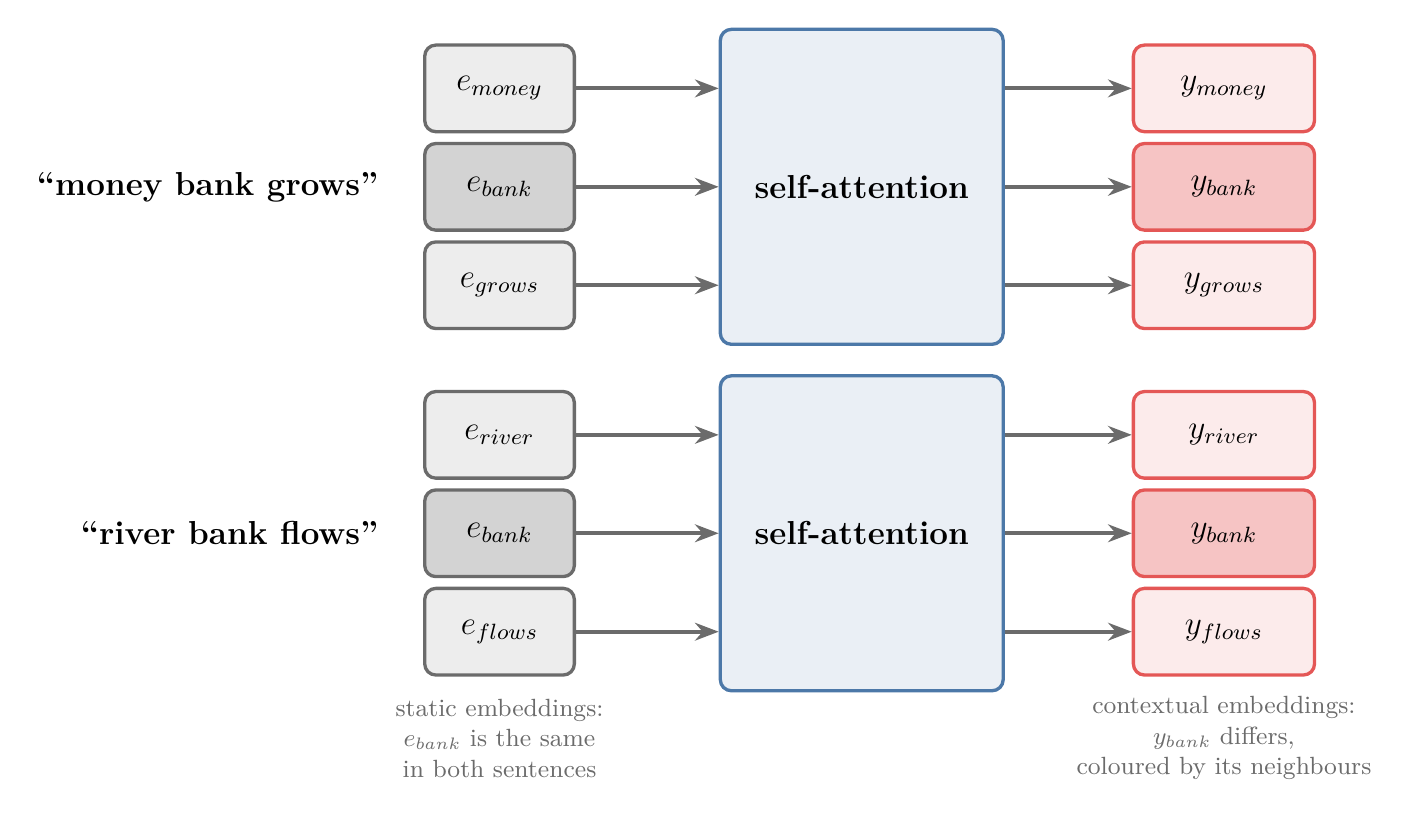
\begin{tikzpicture}[every node/.append style={font=\sffamily\large}]
  \foreach \row/\w/\v/\y in {0/money/grows/0, 1/river/flows/-4.4} {
    \node[box=cgrey, minimum width=1.9cm] (a\row) at (0,\y+1.25) {$e_{\text{\w}}$};
    \node[box=cgrey, minimum width=1.9cm, fill=cgrey!30] (b\row) at (0,\y) {$e_{\text{bank}}$};
    \node[box=cgrey, minimum width=1.9cm] (c\row) at (0,\y-1.25) {$e_{\text{\v}}$};
    \node[box=cblue, text width=3.1cm, minimum height=4.0cm] (sa\row) at (4.6,\y) {\textbf{self-attention}};
    \node[box=cred, minimum width=2.3cm] (x\row) at (9.2,\y+1.25) {$y_{\text{\w}}$};
    \node[box=cred, minimum width=2.3cm, fill=cred!35] (y\row) at (9.2,\y) {$y_{\text{bank}}$};
    \node[box=cred, minimum width=2.3cm] (z\row) at (9.2,\y-1.25) {$y_{\text{\v}}$};
    \foreach \n in {a,b,c} \draw[arrow] (\n\row.east) -- (sa\row.west |- \n\row.east);
    \foreach \n in {x,y,z} \draw[arrow] (sa\row.east |- \n\row.west) -- (\n\row.west);
    \node[font=\sffamily\bfseries\large, anchor=east] at (-1.4,\y) {``\w{} bank \v''};
  }
  \node[note, text width=3.6cm] at (0,-7.0) {static embeddings:\\$e_{\text{bank}}$ is the same\\in both sentences};
  \node[note, text width=3.8cm] at (9.2,-7.0) {contextual embeddings:\\$y_{\text{bank}}$ differs,\\coloured by its neighbours};
\end{tikzpicture}
\end{document}
